\documentclass[aspectratio=169]{beamer}
% packages
\usepackage{multicol}
\usepackage[T2A]{fontenc}
\usepackage[utf8]{inputenc}
\usepackage[english,russian]{babel}
\usepackage{booktabs}
\usepackage{biblatex}
\usepackage{graphicx}
\usepackage{href-ul}
\usepackage{cmap}
\usepackage{svg}

\usepackage{lipsum}

% math packages
\usepackage{amsmath,amsfonts,amssymb,amsthm,mathtools}
\usepackage{mathtext}
\usepackage{icomma}
\usepackage{floatflt}

% settings
\setbeamertemplate{navigation symbols}{}
\setbeamertemplate{section in toc}[sections numbered]
\setlength{\columnseprule}{0.2pt}

%%%%%%%%%%%%%%%%%%%%%%%%%%%%%%%%%%
% Metropolis Theme Configuration %
%%%%%%%%%%%%%%%%%%%%%%%%%%%%%%%%%%

\usetheme[
    %%% main theme %%%
    titleformat=regular, 
    %%% inner theme %%%
    sectionpage=progressbar, % + slide
    %sectionpage=none, % disables section page
    %%% outer theme %%%
    numbering=fraction,
    progressbar=frametitle,
    %%% color theme %%%
    block=transparent,
    background=light
]{metropolis}

%%%%%%%%%%%%% Title %%%%%%%%%%%%%%

\setbeamertemplate{title page}{
  \begin{minipage}[b][\paperheight]{\textwidth}
    \centering  % <-- Center here
    \ifx\inserttitlegraphic\@empty\else\usebeamertemplate*{title graphic}\fi
    \vfill%
    \ifx\inserttitle\@empty\else\usebeamertemplate*{title}\fi
    \ifx\insertsubtitle\@empty\else\usebeamertemplate*{subtitle}\fi
    \usebeamertemplate*{title separator}
    \ifx\beamer@shortauthor\@empty\else\usebeamertemplate*{author}\fi
    \ifx\insertdate\@empty\else\usebeamertemplate*{date}\fi
    \ifx\insertinstitute\@empty\else\usebeamertemplate*{institute}\fi
    \vfill
    \vspace*{1mm}
  \end{minipage}
}

\setbeamertemplate{title}{
%  \raggedright%  % <-- Comment here
  \linespread{1.0}%
  \inserttitle%
  \par%
  \vspace*{0.5em}
}
\setbeamertemplate{subtitle}{
%  \raggedright%  % <-- Comment here
  \insertsubtitle%
  \par%
  \vspace*{0.5em}
}

%%%%%%%%%%%%% Blocks %%%%%%%%%%%%%

% map defaulf block to oldblock
\let\oldblock\block
\let\endoldblock\endblock

% change block by adding smallskip
\renewenvironment{block}[1]
{\begin{oldblock}{#1}
    \smallskip
}
{ 
\end{oldblock}
}

\setbeamerfont{bibliography entry title}{size=}
\setbeamerfont{bibliography entry author}{size=}
\setbeamerfont{bibliography entry location}{size=}
\setbeamerfont{bibliography entry note}{size=}

%%%%%%%%%%%%% Colors %%%%%%%%%%%%%

\setbeamercolor{normal text}{fg=black, bg=white}
\setbeamercolor{progress bar}{fg=normal text.fg, bg=normal text.fg!50!black!30} 
\setbeamercolor{frametitle}{fg=normal text.fg, bg=normal text.bg}

% \definecolor{myblue}{RGB}{52,52,178}
% \setbeamercolor{normal text}{fg=black, bg=white}
% \setbeamercolor{progress bar}{fg=normal text.fg, bg=normal text.fg!50!black!30} 
% \setbeamercolor{frametitle}{fg=myblue, bg=normal text.bg}
% \setbeamercolor{palette primary}{bg=myblue}
% \setbeamercolor{block title}{fg=myblue}
% \setbeamercolor{titlelike}{fg=myblue}
% latin bold lower
\newcommand{\ba}{\mathbf{a}} 
\newcommand{\bc}{\mathbf{c}} 
\newcommand{\be}{\mathbf{e}} 
\newcommand{\bh}{\mathbf{h}} 
\newcommand{\bp}{\mathbf{p}} 
\newcommand{\bt}{\mathbf{t}} 
\newcommand{\bs}{\mathbf{s}} 
\newcommand{\bu}{\mathbf{u}} 
\newcommand{\bv}{\mathbf{v}} 
\newcommand{\bw}{\mathbf{w}} 
\newcommand{\bx}{\mathbf{x}} 
\newcommand{\by}{\mathbf{y}} 
\newcommand{\bz}{\mathbf{z}} 
\newcommand{\bm}{\mathbf{m}} 

% latin bold upper
\newcommand{\bA}{\mathbf{A}} 
\newcommand{\bB}{\mathbf{B}} 
\newcommand{\bC}{\mathbf{C}} 
\newcommand{\bG}{\mathbf{G}}
\newcommand{\bF}{\mathbf{F}}
\newcommand{\bI}{\mathbf{I}} 
\newcommand{\bJ}{\mathbf{J}} 
\newcommand{\bL}{\mathbf{L}} 
\newcommand{\bM}{\mathbf{M}} 
\newcommand{\bH}{\mathbf{H}}
\newcommand{\bP}{\mathbf{P}}
\newcommand{\bQ}{\mathbf{Q}} 
\newcommand{\bR}{\mathbf{R}} 
\newcommand{\bT}{\mathbf{T}} 
\newcommand{\bU}{\mathbf{U}} 
\newcommand{\bV}{\mathbf{V}} 
\newcommand{\bW}{\mathbf{W}} 
\newcommand{\bX}{\mathbf{X}} 
\newcommand{\bY}{\mathbf{Y}} 
\newcommand{\bZ}{\mathbf{Z}} 

% latin cal upper
\newcommand{\cF}{\mathcal{F}} 
\newcommand{\cG}{\mathcal{G}} 
\newcommand{\cI}{\mathcal{I}} 
\newcommand{\cL}{\mathcal{L}} 
\newcommand{\cM}{\mathcal{M}} 
\newcommand{\cN}{\mathcal{N}} 
\newcommand{\cS}{\mathcal{S}} 
\newcommand{\cT}{\mathcal{T}} 
\newcommand{\cW}{\mathcal{W}} 
\newcommand{\cX}{\mathcal{X}} 
\newcommand{\cY}{\mathcal{Y}} 
\newcommand{\cZ}{\mathcal{Z}} 

% latin bb upper
\newcommand{\bbE}{\mathbb{E}} 
\newcommand{\bbI}{\mathbb{I}} 
\newcommand{\bbP}{\mathbb{P}} 
\newcommand{\bbR}{\mathbb{R}}
\newcommand{\bbX}{\mathbb{X}} 
\newcommand{\bbY}{\mathbb{Y}}
\newcommand{\bbW}{\mathbb{W}} 

% greek bold lower
\newcommand{\bLambda}{\boldsymbol{\Lambda}}

\newcommand{\bepsilon}{\boldsymbol{\epsilon}} 
\newcommand{\btheta}{\boldsymbol{\theta}} 
\newcommand{\blambda}{\boldsymbol{\lambda}} 
\newcommand{\bpi}{\boldsymbol{\pi}} 
\newcommand{\bmu}{\boldsymbol{\mu}} 
\newcommand{\bsigma}{\boldsymbol{\sigma}} 
\newcommand{\bphi}{\boldsymbol{\phi}} 

% greek bold upper
\newcommand{\bSigma}{\boldsymbol{\Sigma}} 

% transpose
\newcommand{\T}{^{\text{\tiny\sffamily\upshape\mdseries T}}}

\newcommand{\norm}[1]{\left\|#1\right\|}
% \addbibresource{references.bib}
% \graphicspath{{../isp/figs}
\usefonttheme[onlymath]{serif}
\newcommand\freefootnote[1]{%
  \let\thefootnote\relax%
  \footnotetext{#1}%
  \let\thefootnote\svthefootnote%
}

%%%
\title{Анализ сходимости поверхности функции потерь сверхточных нейросетевых моделей на основе Гессиана}
\author{
    Владислав Мешков, Никита Киселев, Андрей Грабовой\\
}
\date{}
\institute[MIPT]{
    Московский Физико-Технический Институт
}
%%%

\begin{document}

\maketitle

\begin{frame}{Мотивация}
    \begin{block}{Проблема}
    Число данных для обучения нейросетей, а также число параметров растет. Необходимо изучать связь между сложностью моделей и необходимым числом объектов в обучающей выборке.
    \end{block}
    \begin{block}{Цель}
    Изучить сходимость поверхности функции потерь в пространстве параметров при изменении размера выборки для сетей, представленных в виде произведения зависимых от входа матриц.
    \end{block}
    \begin{block}{Решение}
        \begin{enumerate}
        \item[1.] Рассмотреть взаимосвязь гессиана со сходимостью функции потерь.
        \item[2.] Посчитать норму гессиана для сетей, представленных в виде произведения матриц, и применить данные результат к сверточным сетям.
        \end{enumerate}
    \end{block}
\end{frame}

\begin{frame}{Постановка задачи}
    Пусть $f_{\btheta}$~--- нейросеть, $\bx_k$~--- входы, $\by_{k}$~--- one-hot метки классов, $\cL_k$~--- функция потерь на $k$ первых объектах.
    \vspace{-0.75em}
    \begin{block}{Изменение значения при добавлении одного объекта}
    \vspace{-0.5em}
        \begin{equation*}
            \mathcal{L}_{k+1}(\boldsymbol{\theta}) - \mathcal{L}_k(\boldsymbol{\theta}) = \dfrac{1}{k+1} \left( \ell(f_{\boldsymbol{\theta}}(\mathbf{x}_{k+1}), \mathbf{y}_{k+1}) - \mathcal{L}_{k}(\boldsymbol{\theta}) \right)
        \end{equation*}
    \end{block}

    \begin{columns}
        \begin{column}{0.4\textwidth}
            \vspace{1em}
            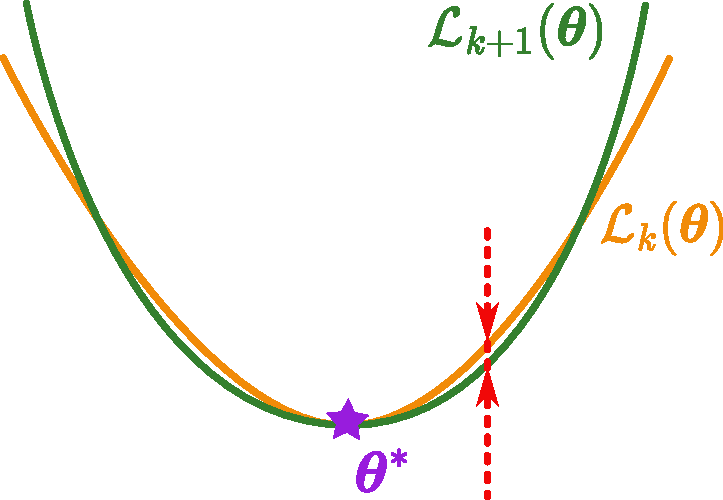
\includegraphics[width=0.95\textwidth]{slides/loss-diff.pdf}    
        \end{column}

        \begin{column}{0.6\textwidth}
        \begin{center}
        \vspace{-2em}
         \begin{block}{Предположение 1}
            \vspace{-0.5em}
            Пусть $\boldsymbol{\theta}^*$ является точкой локального минимума обеих функций $\mathcal{L}_{k}(\boldsymbol{\theta})$ и $\mathcal{L}_{k+1}(\boldsymbol{\theta})$: $\nabla \mathcal{L}_{k}(\boldsymbol{\theta}^*) = \nabla \mathcal{L}_{k+1}(\boldsymbol{\theta}^*) = \mathbf{0}$.
        \end{block}
        \vspace{-0.5em}
        \begin{block}{Аппроксимация второго порядка}
        \vspace{-1.7em}
        \[\mathbf{H}^{(k)} = \dfrac{1}{k} \sum\limits_{i=1}^{k} \mathbf{H}_{i}(\boldsymbol{\theta}) = \dfrac1k \sum\limits_{i=1}^k\nabla_{\btheta}^2\ell(f_{\btheta}(\bx_i), \by_i)\]
        \vspace{-1.0em}
        \begin{equation*}
            \mathcal{L}_{k}(\boldsymbol{\theta}) \approx \mathcal{L}_{k}(\boldsymbol{\theta}^*) + \dfrac{1}{2} (\boldsymbol{\theta} - \boldsymbol{\theta}^*)\T \mathbf{H}^{(k)}(\boldsymbol{\theta}^*) (\boldsymbol{\theta} - \boldsymbol{\theta}^*)
        \end{equation*}
        \vspace{-1.5em}
        \end{block}
        
        \end{center}
        \end{column}
        
    \end{columns}

\end{frame}

%\begin{frame}{Предположение о точке минимума}
%    \begin{block}{Предположение 1}
%        \vspace{-0.5em}
%        Пусть $\boldsymbol{\theta}^*$ является точкой локального минимума обеих функций $\mathcal{L}_{k}(\boldsymbol{\theta})$ и $\mathcal{L}_{k+1}(\boldsymbol{\theta})$, то есть $\nabla \mathcal{L}_{k}(\boldsymbol{\theta}^*) = \nabla \mathcal{L}_{k+1}(\boldsymbol{\theta}^*) = \mathbf{0}$.
%    \end{block}
%    \begin{block}{Аппроксимация второго порядка}
%        \[\bH_i := \nabla_{\btheta}^2\ell(f_{\btheta}(\bx_i), \by_i)\]
%        \[\mathbf{H}^{(k)} = \dfrac{1}{k} \sum\limits_{i=1}^{k} \mathbf{H}_{i}(\boldsymbol{\theta}) \]
%        \vspace{-0.5em}
%        \begin{equation*}
%            \mathcal{L}_{k}(\boldsymbol{\theta}) \approx \mathcal{L}_{k}(\boldsymbol{\theta}^*) + \dfrac{1}{2} (\boldsymbol{\theta} - \boldsymbol{\theta}^*)\T \mathbf{H}^{(k)}(\boldsymbol{\theta}^*) (\boldsymbol{\theta} - \boldsymbol{\theta}^*)
%        \end{equation*}
%    \end{block}
%    \vspace{-1em}
%\end{frame}


\begin{frame}{Связь изменения функции потерь с Гессианом}
    \vspace{-0.7em}
    \begin{block}{Абсолютное изменение функции потерь}
        \vspace{-1em}
        \[\left| \mathcal{L}_{k+1}(\boldsymbol{\theta}) - \mathcal{L}_k(\boldsymbol{\theta}) \right| \leqslant \dfrac{2}{k+1}\max\limits_{i=\overline{1,k+1}} \left|\ell(f_{\btheta^*}(\bx_{i}, \by_{i})) \right| + \]
        \vspace{-1em}
        \[+ \frac{2}{k+1}\norm{\btheta - \btheta^*}^2_2\max\limits_{i=\overline{1,k+1}}{\norm{\bH_{i}(\btheta^*)}}\]
        %\[ \left| \mathcal{L}_{k+1}(\boldsymbol{\theta}) - \mathcal{L}_k(\boldsymbol{\theta}) \right| \leqslant \dfrac{1}{k+1} \left| \ell(f_{\boldsymbol{\theta}^*}(\mathbf{x}_{k+1}), \mathbf{y}_{k+1}) - \dfrac{1}{k} \sum\limits_{i=1}^{k} \ell(f_{\boldsymbol{\theta}^*}(\mathbf{x}_{i}), \mathbf{y}_{i}) \right| + \]
        %\[ + \dfrac{1}{k+1} \left\|\boldsymbol{\theta} - \boldsymbol{\theta}^*\right\|_2^2 \left\| \mathbf{H}_{k+1}(\boldsymbol{\theta}^*) - \dfrac{1}{k} \sum\limits_{i=1}^{k} \mathbf{H}_{i}(\boldsymbol{\theta}^*) \right\|_2 \]
    \end{block}
    \vspace{-1em}
    \begin{block}{Декомпозиция Гессиана}
        \vspace{-1em}
        \[
            \mathbf{H}_{i}(\boldsymbol{\theta}) = \underbrace{\nabla_{\boldsymbol{\theta}} \mathbf{z}_i \dfrac{\partial^2 \ell(\mathbf{z}_i, \mathbf{y}_i)}{\partial \mathbf{z}_{i}^2} \nabla_{\boldsymbol{\theta}} \mathbf{z}_i\T }_{\bH_O} + \underbrace{\sum\limits_{k=1}^{K} \dfrac{\partial \ell(\mathbf{z}_i, \mathbf{y}_i)}{\partial z_{ik}} \nabla^2_{\boldsymbol{\theta}} z_{ik}}_{\bH_F}
        \]
    \end{block}
    \vspace{-2em}
%\end{frame}
%
%
%\begin{frame}{Оценка абсолютного изменения функции потерь Гессианом}
%    \begin{block}{Простое следствие из нер-ва треугольника}
%        
%    \end{block}
    \begin{block}{Аппроксимация Гессиана}
    \begin{itemize}
        \item Аппроксимируем Гессиан, пренебрегая $\bH_F$. В задаче $K$-классовой классификации $\norm{\bH_F}\ll \norm{\bH_O}$
        \item Тогда можно оценить $\norm{\bH} \approx \norm{\bH_O}$.
    \end{itemize}
    \end{block}
\end{frame}

\begin{frame}{Нейросети представимые в виде произведения матриц}
Рассмотрим нейросети специального вида, а именно представимые в виде произведения матриц, возможно зависимых от входа. \\
        Пусть нейросеть $f_{\btheta}(\bx) := \bT^{(L+1)}\bLambda^{(L)}\dots \bLambda^{(1)}\bT^{(1)}\bx$, где 
        \vspace{-0.5em}
        \begin{itemize}
        \item $\bx$~--- вход \item $\bT^{(l)}$~--- матрица линейного слоя $l$
        \item $\bLambda^{(l)}$~--- матрица $ReLU$-активации $l$-го слоя, зависимая от входа $\bx$
        
        \end{itemize}
\end{frame}


\begin{frame}{Структура $\bH_O$ компоненты Гессиана} 
\vspace{-0.5em}
Рассмотрим матрицы:
\begin{itemize}
\item $\bF$~--- матрица сложной структуры, зависящая только от всех $\bT^{(i)}, \bLambda^{(i)}$ и от $\bx$ 
\item $\bA = \mathrm{diag}(\bp) - \bp\bp\T$, где $\bp$~--- вектор вероятностей классов для $\bx$
\item $\bQ^{(p)} := \frac{\partial \bT^{(p)}}{\partial \bW^{(p)}}$, где $\bW^{(p)}$~--- параметры $p$-го слоя.
\vspace{-0.5em}
\end{itemize}
    \begin{block}{Лемма 1}
        $\bH_O(\btheta) = \bQ\T\bF\T\bA\bF\bQ$.
    \end{block}
    Данная Лемма позволяет представить норму $\bH_O$ компоненты Гессиана как произведение норм более простых блоков.
\end{frame}

\begin{frame}{Оценка нормы Гессиана}
    \begin{block}{Лемма 2} 
    \vspace{-0.5em}
    Пусть $\norm{\bQ^{(p)}}_2 \leqslant q, \norm{\bT^{(p)}}^2 \leqslant w_{\bT}^2\;\; \forall p$, тогда \\
    $\norm{\bH_O} \leqslant \sqrt{2}q^2\norm{\bx}^2(L+1)w_{\bT}^{2L}.$
    \end{block}
    Оценка нормы $\bH_O$ как функция весов является степенной, а как функция числа слоев~--- показательной. \\
    \textbf{Лемма 2} является основой для оценки нормы гессиана в дальнейшем. \\
    Из Леммы, для того, чтобы оценить Гессиан, достаточно оценить $\norm{\bQ^{(p)}}$ и $\norm{\bT^{(p)}}$ одновременно для всех слоев, что и будет проделано в будущих результатах.
    
\end{frame}

\begin{frame}{Свертки как линейная операция}
    Действие свертки на $\bx \in \bbR^{C\times d}$ представим линейным оператором, действующим на $\bx \in \bbR^{Cd}$, причем с сохранением обозначений\;\;: $\bT^{(l)}*\bx \rightarrow \bT^{(l)}\bx$ \\
    \begin{align*}
        \begin{pmatrix}
            t_1 & t_2 & t_3
        \end{pmatrix}*
        \begin{pmatrix}
            x_1 \\
            x_2 \\
            x_3 \\
            x_4 \\
            x_5
        \end{pmatrix} \rightarrow
        \begin{pmatrix}
            t_1 & t_2 & t_3 & 0 & 0 \\
            0 & t_1 & t_2 & t_3 & 0 \\
            0 & 0 & t_1 & t_2 & t_3 
        \end{pmatrix}
        \begin{pmatrix}
            x_1 \\
            x_2 \\
            x_3 \\
            x_4 \\
            x_5
        \end{pmatrix}
    \end{align*}
\end{frame}

\begin{frame}{Результаты для 1-D сверток}
\begin{block}{Теорема 1}
    Пусть $C_l \leqslant C,\; k_i \leqslant k, \; d_i \leqslant d, \; |W_{i,j,k}^{(p)}|^2 \leqslant w^2$, где $C_l, k_l, d_l$~--- число каналов, размер ядра и пространственный размер соответственно, тогда \\
    \[\norm{\bH_O} \leqslant \sqrt{2}\norm{x}^2\textcolor{blue}{d^2}(L+1)(\textcolor{blue}{C^2w^2kd})^L\]
\end{block}
Из Теоремы видно, что оценка нормы является степенной функцией от числа каналов, весов, размера ядра и размера последовательности
\end{frame}

\begin{frame}{Результаты для 2-D свеерток}
\begin{block}{Теорема 2}
    Пусть $|\bW^{(p)}_{i,j,k,t}|^2 \leqslant w^2$, где $\bW^{(p)}$~--- веса $p$-го слоя свртки \\
    $C_l, k_l, (m_l, n_l)$~--- число каналов, размер ядра, пространственные размеры карты признаков соответственно на $l$-м слое нейросети.
    Пусть $C_l \leqslant C, \;\; k_i \leqslant k,\; m_i \leqslant m, \;\; n_i \leqslant n$, тогда \\
    \vspace{-0.75em}
    \[\norm{\bH_O} \leqslant \sqrt{2}\norm{x}^2\textcolor{blue}{C^2k^2mn}(L+1)(\textcolor{blue}{C^2k^2w^2mn})^L.\]
\end{block}

Результат полученный в \textbf{Теореме 1} отличается от данного лучшей оценкой $\norm{\bQ^{(p)}}$, это связано с различием в структуре Теплицевых матриц 1D и 2D сверток.

\end{frame}

\begin{frame}{Результаты для пулингов и полносвязной головы}
    \begin{block}{Лемма 3}
        Пусть на месте $l$-й нелинейности находится max/avg пулинг, причем пусть ядро:~$k_{\mathrm{pool}} \times k_{\mathrm{pool}}$, $\textrm{stride}=k_{\mathrm{pool}}, \textrm{padding}=0$, при этом верны все ограничения предыдущей теоремы, тогда: \\
        \vspace{-1.5em}
        \[\norm{\bH_O} \leqslant \sqrt{2}\norm{x}^2q^2\frac{1}{\textcolor{blue}{k_{\mathrm{pool}}^{2(L-l+2)}}}(L+1)(C^2k^2w^2mn)^L\]
    \end{block}
    \vspace{-1.5em}
    \begin{block}{Лемма 4}
        Пусть после сверточных слоев нахожится полносвязная голова размера $P$:
        \vspace{-0.5em}
        \begin{align*}
        & f_{\btheta}{(\bx)} = \bT^{(L+P+1)}\bLambda^{(L+P)} \dots \bLambda^{(L+1)}\bT^{(L+1)}\bLambda^{(L)}\dots \bLambda^{(1)}\bT^{(1)}\bx,
        \end{align*}
        где $\bT^{(L+1+i)}$~--- Линейный слой с параметрами $h_{i}, h_{i+1}$, $\bT^{(r)}$-2D-свертки. Пусть имеют место оценки: $\norm{\bT^{(L+1+i)}_{ij}} \leqslant \tilde{w}$ и $h_p \leqslant h$.Тогда в условиях Теоремы 2 имеем
        \vspace{-2.0em}
        \begin{align*}
        & \norm{\bH_{O}} \leqslant \sqrt{2}\norm{\bx}^2C^2k^2mn\textcolor{blue}{\big(h^2\tilde{w}^2\big)^P}\big(k^2C^2w^2mn\big)^L \times \bigg(\textcolor{blue}{L + 1 + P\frac{h^2\tilde{w}^2}{k^2C^2w^2mn}}\bigg).
        \end{align*}
    \end{block}
\end{frame}

\begin{frame}{Постановка эксперимента}
    \begin{itemize}
        \item \textbf{Задача:} классификация изображений.
        \item \textbf{Выборка:} MNIST, FashionMNIST, CIFAR10.
        \item \textbf{Архитектура:} L-слойная сверточная нейросеть с ReLU активациями.
        \item \textbf{Проверяеые гипотезы:}
        Абсолютная разница функции потерь растет в зависимости от
        \begin{enumerate}
            \item числа сверточных слоев,
            \item размера ядра,
            \item числа фильтров.
        \end{enumerate}
        \item \textbf{Постановка эксперимента}
        \begin{enumerate}
            \item Обучаем модель на полном наборе данных и получаем близкое к оптимальному~$\hat{\boldsymbol{\theta}}$,
            \item Находим для всех $k$: $\left| \mathcal{L}_{k+1}(\hat{\boldsymbol{\theta}}) - \mathcal{L}_k(\hat{\boldsymbol{\theta}}) \right|$ для всех $k = 1, \ldots, m$,
            \item Предыдущий пункт повторяем меняя порядок элементов в выборке.
        \end{enumerate}
    \end{itemize}
\end{frame}

\begin{frame}{Число слоев}
    \begin{figure}[ht]
        \centering
        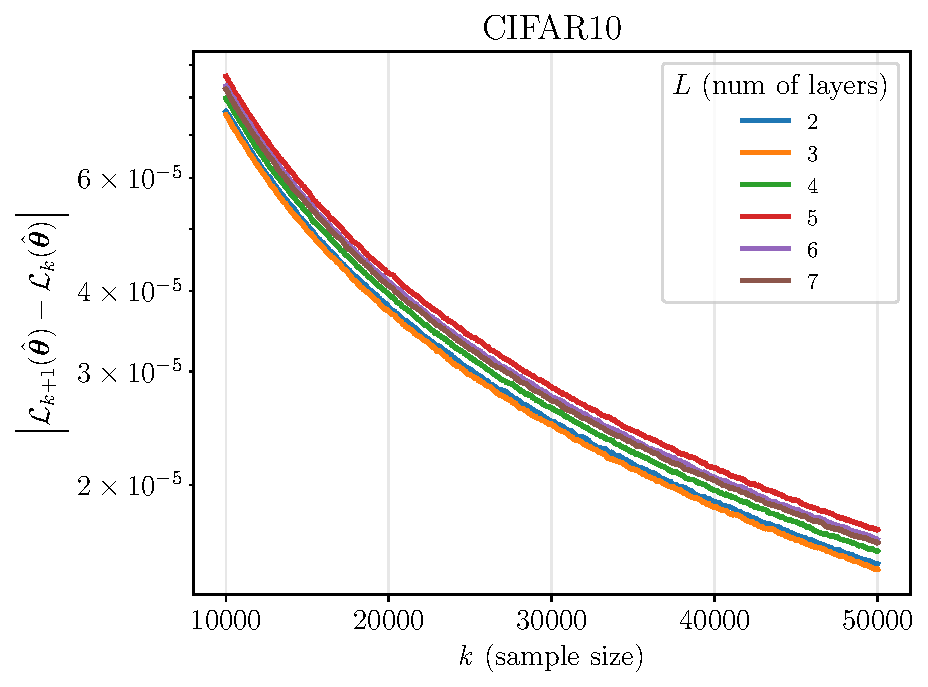
\includegraphics[width=0.5\linewidth]{../isp/figs/cifar10_change_layers.pdf}\hfill
        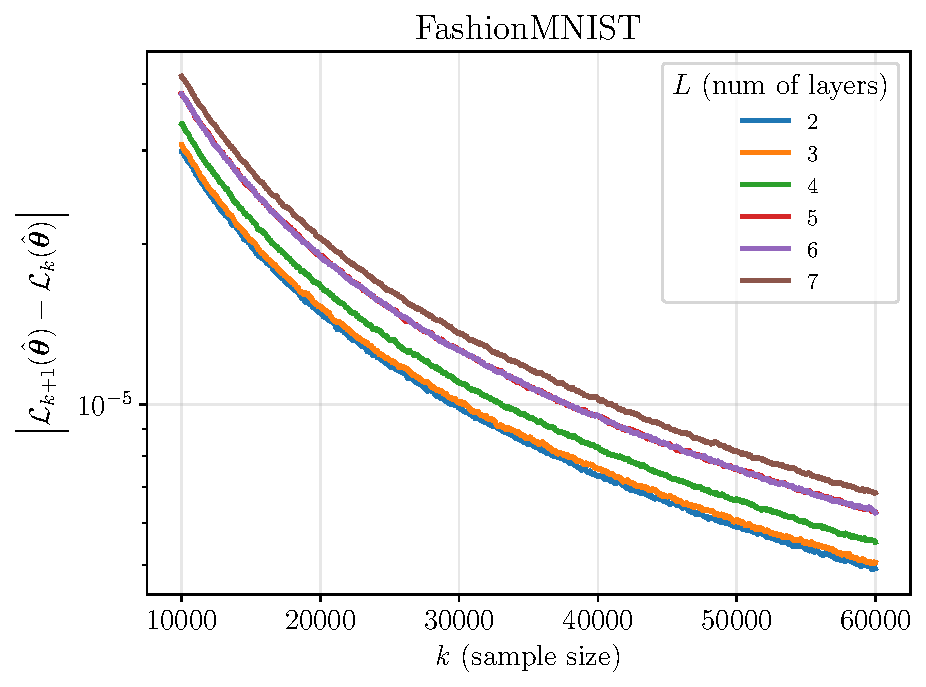
\includegraphics[width=0.5\linewidth]{../isp/figs/fashion_mnist_change_layers.pdf}
        Графики демонстрируют  шумное поведение, но видна тенденция: при увеличении числа слоев абсолютная разница функции потерь также увеличивается.
    \end{figure}
\end{frame}

\begin{frame}{Размер ядра}
    \begin{figure}[ht]
        \centering
        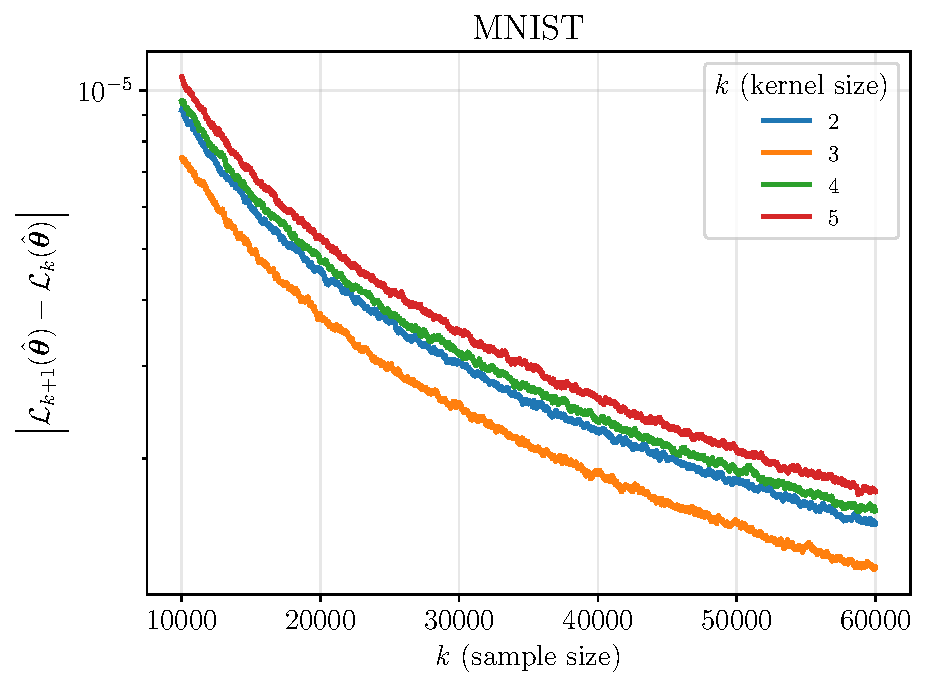
\includegraphics[width=0.5\linewidth]{../isp/figs/mnist_change_kers.pdf}\hfill
        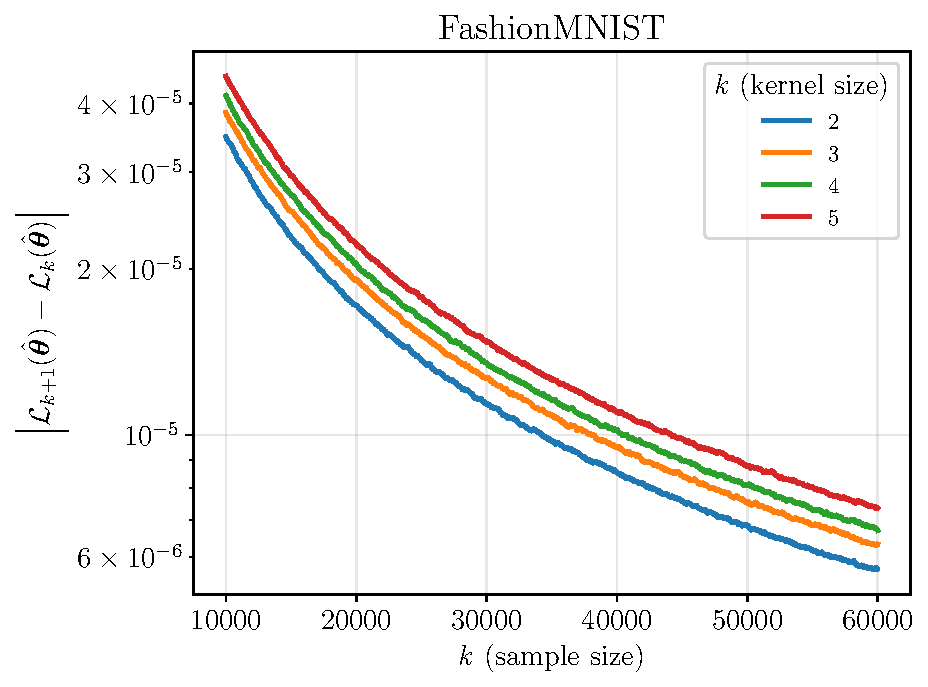
\includegraphics[width=0.5\linewidth]{../isp/figs/fashion_mnist_change_kers.pdf}
        При увеличении размера ядра, абсолютная разница функции потерь также растет.
    \end{figure}
\end{frame}

\begin{frame}{Число фильтров}
    \begin{figure}[ht]
        \centering
        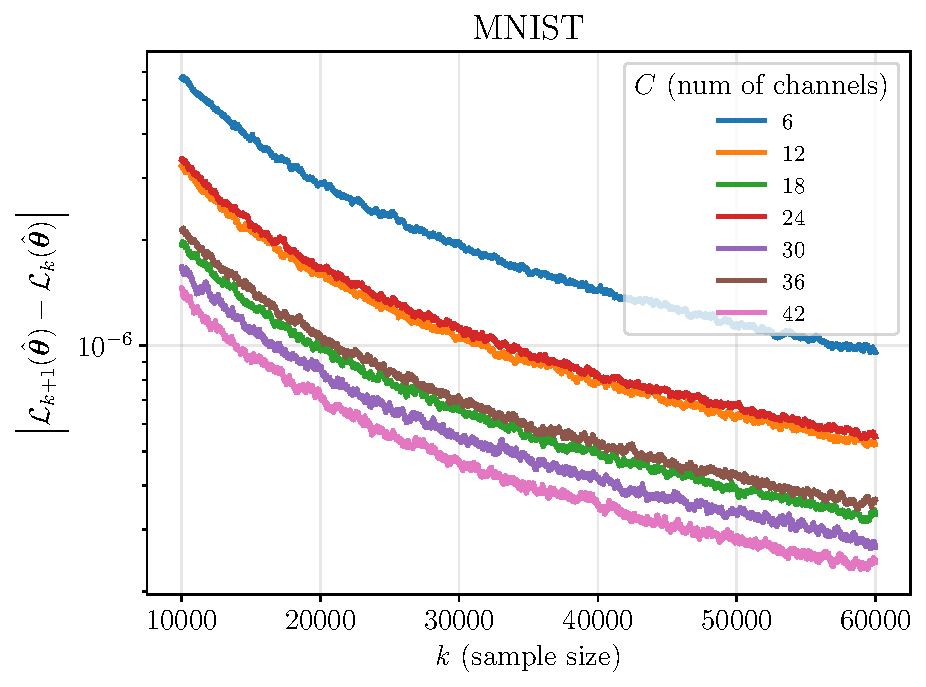
\includegraphics[width=0.5\linewidth]{../isp/figs/mnist_change_channels.pdf}\hfill
        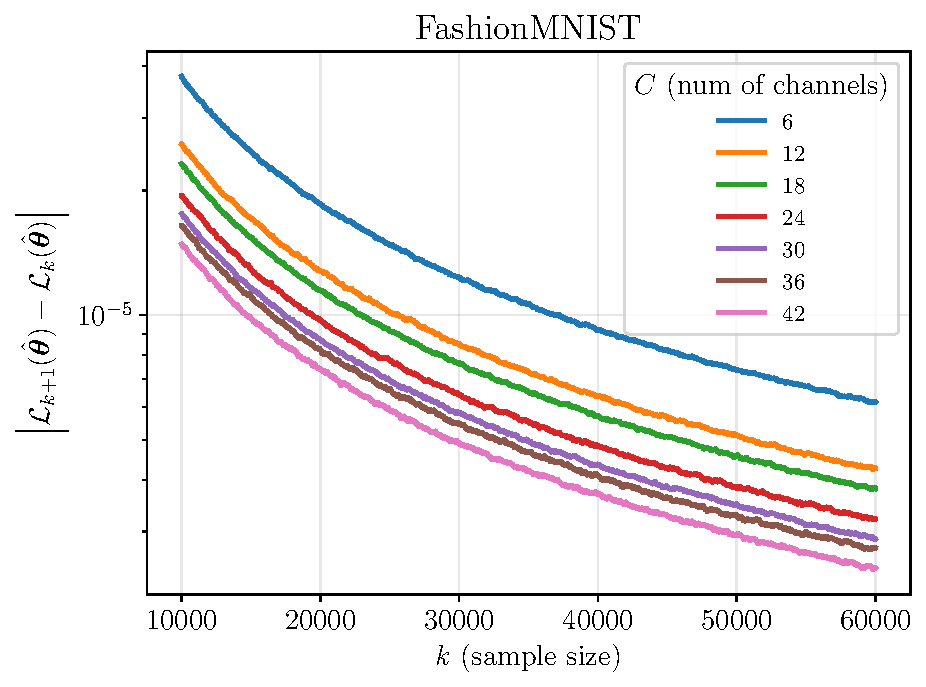
\includegraphics[width=0.5\linewidth]{../isp/figs/fashion_mnist_change_channels.pdf}
        Графики, как видно, демонстрируют обратный результат: при большем числе каналов разница явно меньше. Предположительно, результат таков, так как сети при большем числе фильтров лучше обучились и компонента с Гессианом влияла значимо меньше.
    \end{figure}
\end{frame}

\begin{frame}{Заключение}
    \begin{block}{Основные результаты}
    \begin{enumerate}
        \item Предложен способ оценки нормы гессиана для сетей, представленных в виде произведения матриц.
        \item Данный результат применен для 2D/1D сверток, а также для пулингов и fc-головы.
        \item Предложен способ оценки абсолютной разницы функции потерь для сверточных сетей, основываясь на гессиане.
    \end{enumerate}
    \end{block}
    \vspace{-0.5em}
    
    \begin{block}{Будущее работы}
    \vspace{-0.5em}
    \begin{enumerate}
        \item Улучшить теоретические оценки, пользуясь разреженностью матриц $\bLambda^{(i)}$.
        \item Применить данные оценки к другим видам нейронных сетей.
        \item Проанализировать другие способы оценки изменения ландшафта функции потерь.
    \end{enumerate}
    \end{block}
    \vspace{0.5em}
\end{frame}

\end{document}